\documentclass{article}

\input{handout_preamble}


% ***************************************************
% HEADER INFORMATION

\title{Introduction to Sunray}
\author{The Local Computer Cluster}
\date{}

% ***************************************************

\begin{document}


% ***************************************************
% BEGIN DOCUMENT
% ***************************************************

\maketitle

\begin{center}
    \includegraphics[width=0.5\textwidth]{sun}
\end{center}

\tableofcontents


\newpage


\section{Introduction}

This small guide will help you access the computational resources that are available.
If you are new to running calculations on a cluster system, {\bf read this document thoroughly}.
Especially the section named "Basic workflow".\\

WARNING: If you run a job and allocate more/less resources than the program is using, then this job is wasting resources and time, and will for that reason be {\bf deleted without warning}.


\newpage
\section{The Queue System}

\subsection*{The Queues}

There are a number of nodes (computers) available, and the way we use them is by submitting "jobs"/"calculations" to the queue system.
%
Using this queue system, your job will run when the resources requested are available.
The Sunray cluster is running a job-manager called {\bf SLURM}.
In SLURM a queue is called a partition.\\

There are currently 3 partitions on sunray.

\begin{itemize}
    \item {\bf coms} Primary queue of about 60 nodes, usable by all COMS. \newline
        \code{Intel(R) Xeon(R) 8x CPU X5550 @ 2.67GHz. 48GB RAM}

    \item {\bf sauer} Queue for Stephan Sauer. Consists of 2 Nodes. \newline
        \code{Intel(R) Xeon(R) 12x CPU E5-2640 0 @ 2.50GHz. 128GB RAM}

    \item {\bf comchem} The workstation in C317, mostly for single core calculations for compchem students.

\end{itemize}

\subsection*{The Queue system}

The following SLURM commands will provide you with useful information. Use them.

\begin{lstlisting}
sinfo             # Overview of all the partitions
squeue            # Overview of all queues
squeue -p <part>  # Overview of jobs on specific partition
squeue -u <user>  # Overview of all queues for a specific user
scancel <id>      # Cancel job with jobid <id>
sfree             # Detailed information on free resources and detects possible errors in submissions.
\end{lstlisting}


It is very important, if you have jobs running a long time to check the status of it regularly to see if it is behaving like it should.
Otherwise it is a waste of computational resources.
Especially make sure that the resources the job will use (from the programs input file) is the same as allocated by the queue system (from the submit script). Read carefully next section.\\

\subsection*{Submission scripts}

Template submission scripts for different programs can be found in \code{/opt/bin/submit/}. These templates cannot be modfied by the users!
Copy-paste those you need to your own \code{bin} folder. For example, a user whose username is \code{brian} has his bin directory in \code{/home/brian/bin}.\\

The pre-made scripts are:

\begin{itemize}
\item{submit\_dalton}
\item{submit\_gamess}
\item{submit\_gaussian}
\item{submit\_mopac}
\item{submit\_orca}
\end{itemize}

Let's familiarize with them. The first lines of every submission script are as follow:

\begin{verbatim}

#!/bin/bash

JOB=${1%.*}

SUBMIT=qsub.tmp

PWD=`pwd`

PARTITION=comchem # sauer or coms or comchem
TIME=10:00:00

NCPUS=1
MEM=1gb

\end{verbatim}

The first thing that one may want to change is the \code{PARTITION}, that is which queue to use, as previously described.
Secondly, the time allocated for the job to run. In the reported example, this job would have a maximum of 10 hours to run, not one second more.
If you think/know that your job will require more time, you should change the variable \code{TIME} accordingly.

Thirdly, the number of cpus which will be allocated to the job. Do not get hungry and selfish, try to be considerate of the other users.
However, parallel jobs (that is those running on more than 1 cpu) are usually faster than single cpu jobs, thus freeing resources earlier. You need to
check that your submission script and your input file specify the same numebr of cpus. For example, to launch Gaussian with 2 cpus, one has to add
\code{\%nprocshare=2} at the beginning of the input file, and use \code{NCPUS=2} in their own gaussian submission script.

Finally, the amount of memory is indicated by the variable \code{MEM}. Again, you should align your input and submission files.
For example, in Gaussian the default allocated memory is 256 MB. To specify, e.g., 1 GB in the input file, you should use \code{\%mem=1GB}.

\newpage


\section{Essential Terminal Commands}

You will without a doubt be using a commandline interface when working with sunray.
If you are new to using Linux and a command shell here is a list of the essential commands you cannot live without.
A good idea is also to get a copy of a commandline cheatsheet for linux.\\

\begin{itemize}

    \item \code{\bf cd} changes directory. Change the directory by writing
\begin{lstlisting}
cd directory_name
\end{lstlisting}

        if you want to move up on directory the command is
\begin{lstlisting}
cd ..
\end{lstlisting}

    \item \code{\bf ls} lists current directory. Prints out a list of all the items in the current folder.
    
    \item \code{\bf pwd} shows the current directory
    
    \item \code{\bf cp} copies a file. To copy file1 to file2 use
\begin{lstlisting}
cp file1 file2
\end{lstlisting}
Either files can be specified with their full path:
\begin{lstlisting}
cp /home/username/directory_name1/file1 /home/username/directory_name2/file2
\end{lstlisting}

    \item \code{\bf grep} search for text in file/files. Prints out the search results. If for example you want to find all the optimization steps in a GAMESS output file the command is
\begin{lstlisting}
grep "NSERCH: " filename.log
\end{lstlisting}
        or if you have a set of GAMESS calculations running and you want to know which are completed
\begin{lstlisting}
grep "exited:" *.log
\end{lstlisting}

    \item \code{\bf tail} prints out the last lines of a file. 
        If you are running a calculation and you want to check how far the calculations has gone you can print out the last lines with
\begin{lstlisting}
tail filename.log
\end{lstlisting}

    \item \code{\bf less} read current file. If you want to read a log file, sometimes this is not possible by normal text editors because the log files are so big. For this you can use less and navigate the file via terminal.
\begin{lstlisting}
less filename.log
\end{lstlisting}
    you exit by pressing "q".

    \item \code{\bf vim} if you want to edit files via the terminal you can use vim. 
\begin{lstlisting}
vi filename.inp
\end{lstlisting}
using vim like a boss, you'll need a lot of time, but the most important things to remember is to be in insert mode when you want to write (press "i"), and to exit you need to be in command-mode (press "esc" to exit insert mode) and write \code{:wq} + enter.

\end{itemize}

\newpage
\section{Accessing Sunray}

If you want to work from home the ssh address for sunray is

\begin{lstlisting}
ssh username@sunray.theory.ki.ku.dk
\end{lstlisting}

If you want to be able to open windows (such as gaussview) from home, you can set the flags

\begin{lstlisting}
ssh -XC username@sunray.theory.ki.ku.dk
\end{lstlisting}

to start a X server and forward the visual from sunray.

% TODO sshfs information



\subsection{Access from Windows}

To access sunray from a windows machine you need to download the program PuTTY. It can be found at \url{http://www.chiark.greenend.org.uk/~sgtatham/putty/download.html}.\\

To access the X server you need to install a X-server on windows.
A possible option is the program Xming, which can be downloaded from \url{http://www.straightrunning.com/XmingNotes/}. The 'Public Domain Releases' are for free.
Moreover, Xming is quite well integrated with PuTTY. Follow the instractions on the web page.


\subsection{Access from OS X}

To use the X Server on a Mac with OS X 10.8 or newer, you need to install \emph{XQuartz}.
You can download it at \url{http://xquartz.macosforge.org/}.
At the time of writing (August, 2016) the current version is XQuartz-2.7.9.
Download and install that.
Finally you need to restart your computer for the changes to take effect.
However, you may still experience problems with visualizing remote graphical programs.
You will need to follow the instructions in \url{https://bugs.freedesktop.org/show_bug.cgi?id=96260/}.
In practice, one has to modify the startx file using \code{sudo vi /usr/X11R6/bin/startx}.
Add some code around lines 80 and 107, as described in the attachement patch\_file\_for\_startx from the same web page (the lines starting with a plus sign +).
Finally, you have to give the following command \code{defaults write org.macosforge.xquartz.X11 enable\_iglx -bool true} in your terminal.


\newpage
\section{Folder structure and available software}

Some of the available software (most of the software needed for calculations, such as gaussview) is installed in the /opt/ folder.
For advanced users; please add the /opt/bin/ folder to your \code{\$PATH}.\\

\subsection*{List users}

To get a list of all users on the sunray system write the following in the terminal;

\begin{lstlisting}
sunset_user_view
\end{lstlisting}


Depending on who your supervisor is (be it in the Computational Chemistry course or otherwise), you are going to carry out your calculations in different programs.
The different programs requires different syntax and keywords in the input file.\\

\subsection*{Avogadro}

Avogadro is an open source software tool which can prepare input files for many of the programs you'll encounter and can also visualize the molecular structure of the molecule.
You will find Avogadro under Application $\rightarrow$ Science.
It is easy to draw molecules (and minimize while you draw using the AutoOpt tool) and to prepare input files using the built in editors.

\subsection*{gaussview}

If you're following Computational Chemistry, you will use gaussview a lot during the course.
It works similar to Avogadro but contains some alternate tools and will only prepare input files for the Gaussian program.
To start gaussview open a terminal a write
\begin{lstlisting}
gaussview &
\end{lstlisting}

the "\&" character makes sure the terminal is not locked to the program, so you can use it for other things as well.


\subsection*{Inputfile preparation}

Avogadro and gaussview are great at drawing the molecules, but if you want to export a structure to another program, or if you have the structure in a XYZ format, you can easily convert by using {\bf OpenBabel}.

To convert a file in XYZ format to a GAMESS input file
\begin{lstlisting}
babel -ixyz filename.xyz -ogamin filename.inp
\end{lstlisting}

to get the list for input and output formats write

\begin{lstlisting}
babel -L formats
\end{lstlisting}

If you are working with a lot of files that needs to be converted from XYZ to a specific input format, you can have a header file \code{gamess\_opt} and convert all XYZ-files in a folder like this;

\begin{lstlisting}
for x in *.xyz; do babel -ixyz $x -ogamin ${x%.*}.inp -xf gamess_opt; done
\end{lstlisting}

\newpage
\section{Basic Work Flow}

\begin{center}
\bf Basically; Think Before Submission
\end{center}

% TODO costs -> power / cooling
% TODO CO2
% TODO translate to points


Here is a recommended work flow when working with computations in general.
Follow this, and the number of recalculations you have to make is guaranteed lower than one who does not follow these recommendations.\\

A very first important point is to realize what you want to do.
You've probably been assigned a molecule, so what properties are you interested in?
Is it a basisset analysis?
Do you need to see the effect of using correlation?\\

Once you have that in place, you can start to think about in which order the calculations will be carried out.
A general rule of thumb is that you work your way through one molecule in a serial manner, i.e. no more than one calculation at a time.\\

Until you have a clear idea about what is going on from start all the way to finish, there is no point to have a lot of calculations running because there will be errors and you'll have to correct them.
You don't need to start with the final molecule of interest.
Make a small example system so the calculations will run faster and you can check the output and correct errors that may arise.
Say you have 10 jobs, each taking 50 hours and all of them fail after 40 because you forgot a keyword.
That is 400 hours (17 days!!) of wasted computer time, that others could have used.\\

If you run your jobs parallelized, then you have to be aware of how your computation time scales with the number of cpu's.
It is a waste of resources to run a job on 8 cpu's if the benefit over running it on 4 is marginal.\\

When optimizing your structures it is generally a good idea to use a fast method (like PM6) to get a crude optimized structure, before trying to optimize it with a more computational heavy method.\\

Make sure that you use symmetry in your calculations whenever it is possible!
Your calculation time can scale up to the degrees of freedom squared, so make absolutely sure that you don't waste resources and check if small changes can be made to your structure to enforce symmetry.\\

When doing parallelized calculations, always use 2, 4, 8 etc. cpu's unless having a good reason not to.
Requesting 3 or 5 cpu's often leaves 1-2 cpu's unused on the node.\\

A second important point is that you need to be organized.
Make folders, sub folders so you are always able to find your data files – it happens that you need to find it later on.
Keep a log (be it a document on the computer or a logbook like in a real lab) to help you.\\

Lastly, when you have all you calculations ready for computation, be considerate about others.
You might need to finish 10000 calculations, but do you need to process them all right now?
The case is usually, that no matter how many calculations one have, it is always the collection of data/writing down stuff for the report which take the longest time to finish.
Find a sweet spot between what you can process and you make the rest of the crowd pleased.\\


\newpage
\section{Steno}

Small section on the steno partitions  and what the different partitions are good for.

\subsection*{Partitions}

\begin{itemize}

    \item {\bf kemi3} \code{Intel }
        For large (24 cores) parallelized jobs.
        kemi3 is at least a factor of 1.5 slower than the other partitions, but it has 24 cpu's per node, and is therefore well suited for calculations with near linear scaling.
        This is not a good partition to run single-core DFT calculations on.

    \item {\bf kemi4} \code{Intel }
        For mid-high memory jobs.
        kemi4 has 96gb memory available for 12 cpu's and 2.8 TB harddrive.
        For this reason the node should primarilly be used if a lot of storage is required
        during the job (large mp2/ccsd/cholesky decomposition)

    \item {\bf chem} \code{Intel }
        For mid-high memory jobs.
        chem has 128gb memory available for 12 cpu's and 1.6 TB harddrive.

\end{itemize}

\section{Cheat sheets}

\begin{center}
    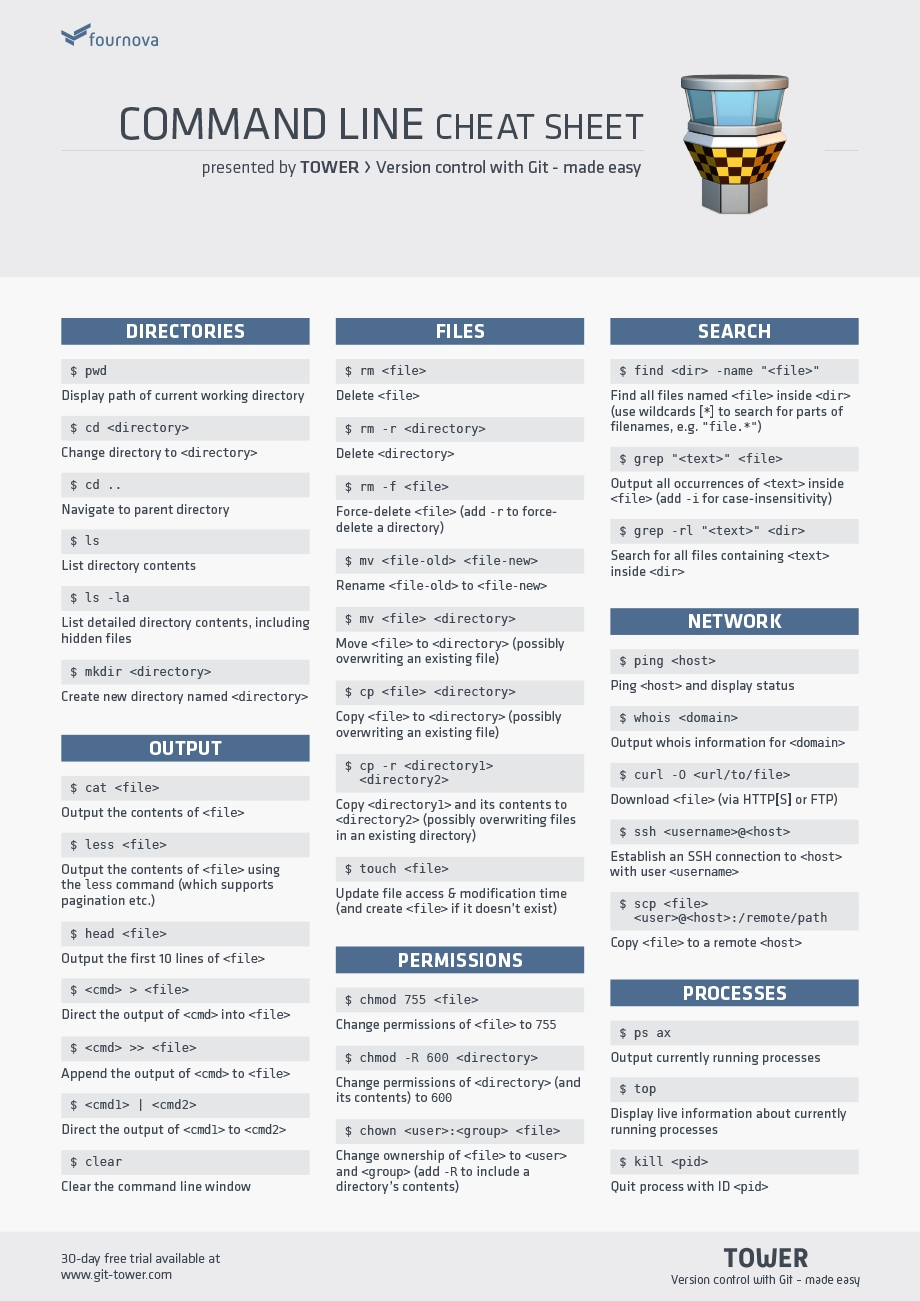
\includegraphics[width=0.95\textwidth]{command-line-cheat-sheet}
\end{center}

\begin{center}
    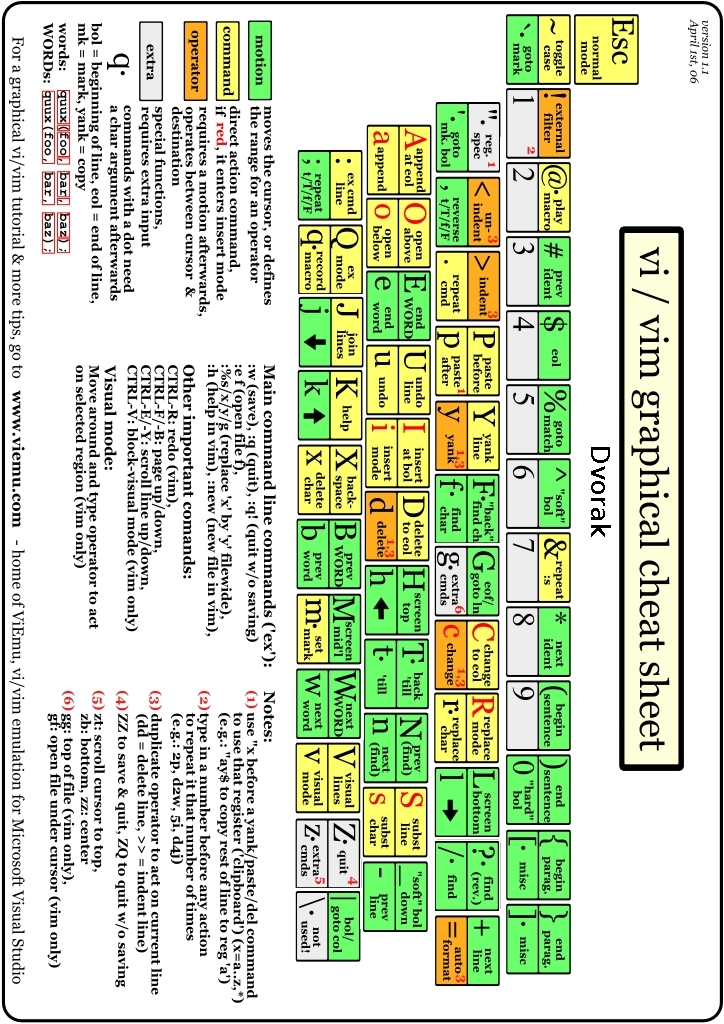
\includegraphics[width=0.95\textwidth]{vim-cheat-sheet}
\end{center}


% ***************************************************
% END DOCUMENT
% ***************************************************

\end{document}
